\documentclass{report} %TODO change
\usepackage{pifont}
\usepackage{natbib}
\usepackage{linguex}
\usepackage{graphicx}

\author{Presley Pizzo}
\title{Properties of a Phonotactic Theory}
\begin{document}

\maketitle

\chapter{Introduction}
The goal of this dissertation is to lay groundwork for the further study of phonotactics.
In Chapter 1, I discuss software that will facilitate the implementation of phonotactic
experiments. In Chapter 2, I review literature that suggests that any accurate model of
phonotactics must allow for the accumulation of violations, so that the grammaticality of
a word depends on all of the violations it contains. I present an experiment with the
ability to refine this statement by investigating how additional violations affect the
grammaticality of the word, weighing on the question of whether linear Harmonic Grammar
or Maximum Entropy grammar is a better model for phonotactics.
In Chapter 3, I ask whether variables not usually considered could affect phonotactics and
need to be included in future modeling. First, I consider that token frequency might correlate
negatively with the weight of a constraint in a grammar, rather than being unrelated. Second,
I consider whether a constraint may have a higher weight in the phonotactic grammar if it is
active in alternations than if it is not. Thus, the dissertation does not propose a particular
model of phonotactics, but aims to narrow the space of models that need to be considered
in the future via empirical investigation, and increase the speed and accuracy of future experimental work in the field.




\chapter{Speriment}
SurveyMan is a desktop application that communicates with Amazon's Mechanical
Turk survey-running website in order to manage surveys and experiments with
minimal human intervention. A working prototype exists but it has many
shortcomings, particularly for linguistics experiments which often have very
precise requirements. I propose to develop an experiment-specific version of
the software that will meet the needs of our phonotactic and psycholinguistic
web-based studies. This would benefit my own research and that of
any linguist interested in running word or sentence judgment studies on the
internet. Other social scientists would also be likely to find it useful.

%TODO make tables out of prose for exp. materials and maybe also software comparison
%IbexFarm either can or will be able to do audio
%Brian Smith used IbexFarm
%write out about control flow
%map out dependencies
This software would enable researchers without a programming background
to set a wide variety of options on the mechanics and presentation of their
experiments.

There are several existing programs to help researchers run experiments on the web, and they differ
from SurveyMan in various ways.

Survey programs like SurveyMonkey and LimeSurvey are relatively easy to use, but lack some
crucial experiment-centric features. In SurveyMonkey, randomization requires a premium membership,
and neither of them handle Latin square designs for the experimenter.

There are also experiment-running programs developed by scientists, such as \citet{WebExp}, \citet{Experigen},
and \citet{PsiTurk}. These tend to require more programming but have more of the features needed for experiments.
However, they still lack some of the features planned for SurveyMan. WebExp, for instance, lacks support for
acoustic stimuli and constrained randomization of question order. Experigen does not record reaction time. PsiTurk
is compatible with any of these features, but the experimenter has to be able to write JavaScript.

\citet{IbexFarm} is a strong candidate for use in web experiments, as it was designed for linguists and thus addresses
most of the features needed for our experiments. However, SurveyMan has plans for advanced features, such as training
periods that continue until the participant performs well enough to advance.

Thus, SurveyMan will balance the ability to design experiments quickly and easily with minimal programming knowledge
with a wide array of features tailored to the needs of phonologists and other social scientists.
% Many other software packages for web-based experiments \citep{WebExp,Experigen,PsiTurk}
% require researchers to run experiments on their own server, which increases
% barriers to access, but SurveyMan will send experiments directly to Mechanical Turk,
% although the option to use one's own server is also in the works. IbexFarm \citep{IbexFarm} is
% another option that hosts experiments for researchers, but SurveyMan will have features
% that IbexFarm lacks in terms of the ease with which researchers can use resources of
% various types and create complex control flow within their experiments.
% Thus, SurveyMan would increase the accessibility of web-based experiments and
% thus the rate at which experiments can be completed.

% Second, the planned version of SurveyMan will tackle an important outstanding
% question in experimental methods, namely how experimenters ought to determine
% the number of participants they need for an experiment to have sufficient
% power.  The practice of running statistical tests on the data in the middle of
% an experiment and adding participants if the results are not yet significant is
% known to distort results \citep{Armitage1969,Snoop,Simmons2011}, and the
% preferred method of deciding on a sample size is to do a power analysis before
% running the experiment based on the effect size found in previous related
% studies. However, if the effect has not previously been studied, it is
% difficult to choose a sample size appropriately. Some techniques have been
% developed to solve this problem \citep{Todd2001}, %TODO bootstrapping
% and we plan to incorporate them directly into the experimental software so that
% participants are added until the program determines that the distribution has
% stabilized.  This feature has the potential to increase the validity of data
% published in the field.

% Thus, this software could benefit research in phonology and other social sciences
% in terms of both quantity and quality.


% \begin{table}
%     \begin{tabular}[h][ccc]
%         Software & Externally Hosted & Latin Square & Resources & Randomization & Branching & Training Loops & Reaction Times \\
%         SurveyMonkey & \ding{51} & & \ding{51} & \ding{51}* & \ding{51}* &  & \\
%         LimeSurvey & \ding{51} & & \ding{51} & \ding{51} & \ding{51} &  & \\
%         WebExp & &  & \ding{51} & \ding{51} & & & \\
%         Experigen & & & \ding{51} & \ding{51} & & & \\
%         PsiTurk & & \ding{51} & & & & \\
%         IbexFarm & \ding{51} & \ding{51} & \ding{51} & \ding{51} && &\\
%         SurveyMan & \ding{51} & \ding{51} & \ding{51} & \ding{51} & \ding{51} & \ding{51} & \ding{51}\\
%     \end{tabular}
% \end{table}

% *Available in premium version.
% **Allows users to write this themselves but does not provide it.

\subsection{Plan}
In order to make an experimental version of SurveyMan that is fully functional
for word and sentence judgment studies, the following features need to be added:

\begin{itemize}
\item Pseudorandomization as an alternative to pure randomization of question order.
\item Counterbalancing of question types.
% \item Statistics to determine optimal sample size.
% \item Reverse qualifications to keep the same participant from taking the experiment
%     more than once. This has already been implemented.
% \item Ability to show multiple resources (images, sounds, or videos) with a question.
%   This is already possible because questions now take arbitrary HTML.
\item Logging of reaction times and the times of events such as playing sounds or videos.
\item Ability to place restrictions on events; for instance, allowing a sound to be played
only once or allowing a choice to be made only after the sound has played.
\item Training loops.
\item Ability to randomly pair images, audio, and video with questions for each participant.
% \item Ability to change the layout of elements on the page.
\end{itemize}

% Additionally, there are changes we would like to make that are not strictly necessary
% but would make the program more extensible and user-friendly:

% \begin{itemize}
% \item Rewrite the software in Python, both for speed of programming and interoperability
% with R.
% \item Create an R interface for the program to replace the current interface (we are currently
%     starting with a Python interface which will make an R interface possible later).
% \item Use a feedback loop to allow experimenters to interact with pilot studies and
% develop experimental designs iteratively.
% \item Set up a JavaScript library to hold user-submitted functions to extend the functionality
% of the software.
% \end{itemize}

Currently, Emma Tosch is working on the backend of the survey-based version of SurveyMan and Molly McMahon is writing a Python front-end,
which will enable an R interface later on. I will adapt SurveyMan to include the necessary experiment-based
features.

I have implemented all of the features necessary to run my own experiments, and will focus on integrating
those changes with the broader SurveyMan framework before adding additional features.




\chapter{Experiment 1: Cumulativity of Violations}
\subsection{Motivation}
% One of the goals of phonology is to develop predictive models of phonotactics.
% Such models predict phonotactic judgments of words based on various properties
% of those words, UG, and the language's lexicon. In order to enable us to choose
% more effective models, I propose to investigate the correlation between the
% number of phonotactic violations in a word and the phonotactic judgment it
% elicits.

In modeling constraint-based phonotactics, there are three broad kinds of decisions to be made: which framework
to use, which parameters (constraints) to use, and how to tune (rank or weight) the parameters. This experiment
aims to offer support for a particular framework, freeing up phonologists to focus on the latter decisions.

Popular constraint-based frameworks include Optimality Theory \citep{Prince1993/2004}, Harmonic Grammar (taken here to mean linear Harmonic
Grammar, in which harmony scores are not subject to exponentiation) \citep{Legendre1990c,Smolensky2006b,Pater2009,Potts2010}, and Maximum Entropy
\citep{Goldwater2003}.



%Ohala and Ohala 1986

% It may be linear, so that each additional violation of equal
% magnitude decreases judgments equally, or it may be nonlinear, so that
% additional violations have increasing or decreasing contributions to judgments.

Optimality Theory predicts that adding mild
violations to a word with a severe violation has no effect, so that the
function from number of violations to grammaticality is flat for any given
first violation as long as it remains one of the worst violations in the word.

However, predating OT, \citet{Ohala1986} found that speakers have an above
chance probability of preferring a word with one violation to a word with that
same violation and a less severe one, suggesting that even the milder violations
affect the grammaticality of a word. Additionally, \citet{Coleman1997} found
that a word like \textit{mrupation}, with one severe violation followed by a
common English sequence, was preferred to a word like \textit{spleitisak}, with
several minor violations.  \citet{Albright_clusters_2008} designed experiments
to directly test the question of cumulativity of violations, addressing
potential alternative explanations for these two results, and found that models
that take into account all violations of a word, not just its worst violation,
fit the data significantly better.

%Sorace and Keller 2004 found cumulativity of violations for syntax
%TODO discuss grammaticality vs acceptability vs ratings

However, Albright did not compare various cumulative models against each other.
The shape of the curve relating number of violations to phonotactic judgments
bears on the question of which framework we should use to model phonotactic
well-formedness. As \citet{Pater_cumulative_2008} points out, Harmonic Grammar
predicts a well-restricted set of cumulativity effects, unlike Optimality
Theory with Local Constraint Conjunction \citep{Smolensky2006d}.
But the weighted constraints of Harmonic Grammar can be combined in a linear fashion,
producing the framework commonly associated with the name, or exponentiated and normalized,
as in Maximum Entropy. These approaches predict differently shaped curves.

\ex. Harmonic Grammar: The harmony $\mathcal{H}$ of a word $x$ is the dot product of the violation vector $v$,
representing violations of $x$ on each constraint in the constraint set $C$, with the constraint
weight vector $w$.\\
\[\mathcal{H}(x) = \sum_{i \in C}{v_iw_i}\]

\ex. Maximum Entropy: The probability $p$ of a word $x$ is the exponentiated negative harmony
of the word, normalized relative to the candidate set $X$.\\
\[p(x_i) = \frac{\exp(-\mathcal{H}(x_i))}{\sum_{j \in X}{\exp(-\mathcal{H}(x_j))}}\]

Consider a constraint with a weight
of two and candidates A, B, C, and D that violate it zero, one, two, and three
times respectively. In linear Harmonic Grammar, the candidates have the harmony scores
0, -2, -4, and -6; they decrease by two each time, in a linear pattern. In
Maximum Entropy, if we assume these candidates exhaust the possibilities, they
have the probabilities 0.865, 0.117, 0.015, and 0.002; candidate A has the
majority of the probability because it is the best choice available, and each
additional violation decreases the probability by a smaller amount than the
last.

\ex. 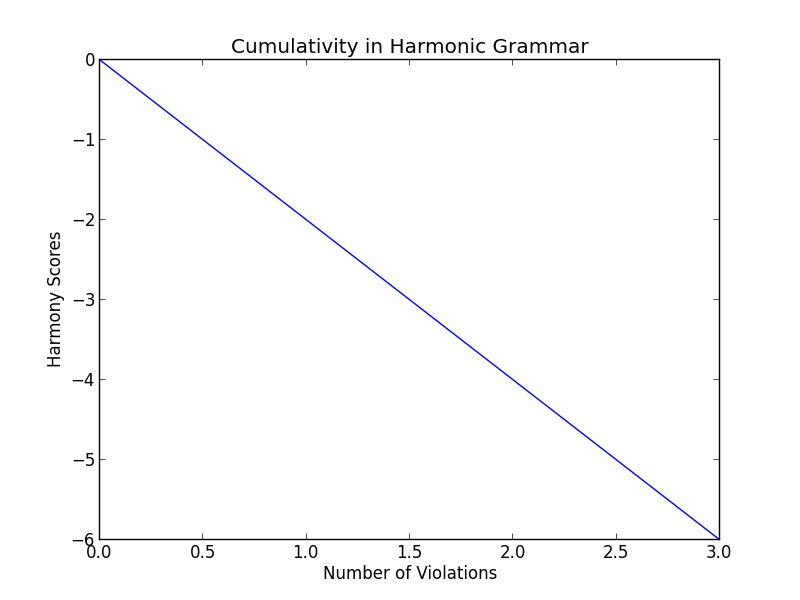
\includegraphics[scale=.5]{hg_cumulativity.png}

\ex. 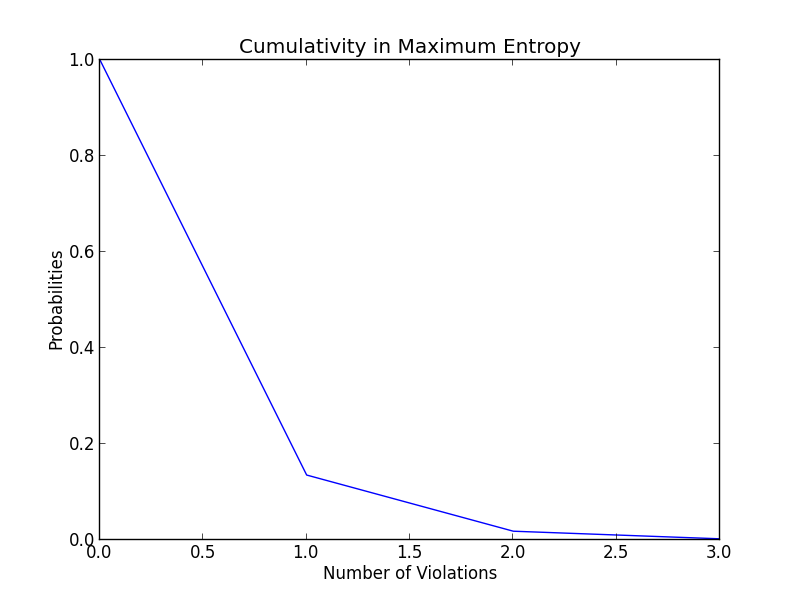
\includegraphics[scale=.5]{me_cumulativity.png}

I predict that, in accordance with the Maximum Entropy model, additional violations
will have smaller effects on the grammaticality of the word, as the grammaticality approaches a floor.


%In order to simplify this investigation, I will not attempt to define the set of patterns
%that can be considered phonotactic violations. Rather, I will use controlled experiments
%dealing only with patterns that are widely accepted to belong to that set for the language
%in question.

\subsection{Plan}

\citet{Albright_clusters_2008} has shown that cumulative models of phonotactics fit data
better than noncumulative ones. He used two types of words, those with
phonotactic violations in the onset and those with phonotactic violations in
the onset as well as milder violatinos in the rime. In a variety of analyses,
he fitted models that rate words by their worst violation only, and ones that
rate words by the sum of all their violations. The models that take into
account all violations in the word were more strongly correlated with experimental
findings. This study showed that cumulative models reflect speaker judgments better
than noncumulative models, but did not distinguish among various cumulative models.

I will ask which kind of cumulative model best fits the data.  Relative to
words with one violation, does the same violation add less, the same amount, or
more ungrammaticality to the word when it appears in a word that already has
another violation?

Each of 24 test items will appear in four conditions. The four conditions are created by
crossing two factors: presence of an onset violation and presence of a rime
violation.  Within an item, the onset violation will be the same whenever it is
present, and likewise for the rime violation. This way, comparing an item with
an onset violation only to the same item with both violations directly shows
the effect of the rime violation. The vowel is held constant across all conditions of an item.

Aside from test items, there will also be filler items. These will be nonce words
of medium acceptability; they will have mild violations that are different from the
kinds of violations found in the test words. Instead of violating cluster phonotactics,
they will violate long-distance OCP constraints or constraints on the cooccurrence of certain
vowels and codas. The goal is to keep participants from comparing filler and test items
piecewise and encourage them to use the filler only to get a sense of a baseline of grammaticality
against which to compare the test words. Fillers will be paired with sets of test items in a way
that minimizes overlap of OCP violating segments with test word segments.
%Participants will be asked to rate these words on a scale from one to four, as
%even-numbered scales allow for better detection of participants that are
%answering randomly.

Participants will be shown pairs of items and asked to choose the one that sounds
more like a possible word of English. Pairs will be composed of one of the test items
and one of the filler items. For each test item, each of its conditions will be compared
against the same set of filler items. A given participant will only see one of these pairings
for each item and filler word, thanks to a Latin Square design.

A mixed effects model will be fitted to the results. The dependent variable
will be proportion of times the test item was chosen. OnsetViolation,
RimeViolation, and their interaction will serve as fixed effects in addition
to random effects for subject and item. % separately for test item and filler item?

The purpose of the experiment is to test whether an interaction exists between
the two fixed effects. Bayesian methods will be used in the case of a null effect
to determine whether the absence of a significant interaction is likely to represent
a truly linear relationship as violations are added.

If a positive interaction is present, this would support a model that takes probability
away from words in greater and greater amounts as the number of violations increases.
I do not know of such a model, and this result is not predicted.

A negative interaction would support models like Maximum Entropy, in which each additional
violation subtracts less probability from the word than the last violation did.

A linear relationship would support models like linear Harmonic Grammar, in which each
additional violation subtracts the same amount of probability from a word as the last
violation did.


% another experiment: what do preference proportions (analogous to ratings) mean?
% - ratings on a scale are hard to interpret
% - proportions taken from 2afc tasks are better - more sensitive, more explicit
% - but still, what do they represent? how reliable are they?
% - do you pick A over B with a ratio of (ratio of A over C / ratio of B over C)?
% - if not, what does that mean?



\chapter{Experiment 2: Effect of Alternations on Phonotactics}
The previous section asked the question, given that words with certain
characteristics are preferred to words with other characteristics, how do those
preferences interact? This chapter will back up and investigate which characteristics
create that difference in the first place. I will assume a baseline
of Maximum Entropy phonotactics, where the type frequency of a sound sequence
correlates with weights on constraints referring to it and thus with its
predicted grammaticality in the language.  In addition to type frequency, other
information about a sound sequence may predict its effect on the grammar.  I
will look for effects of the token frequency of the words the sequence appears
in and whether the pattern is eliminated or produced as a result of a
morphological alternation.

\subsection{Alternations}

% never mind, bad motivation for this project
%As (cite Hayes et al, Becker et al) have shown, some sound sequences that are statistically
%over- or under-represented in the lexicon of a language do not affect judgments in
%experiments. In other words, constraints that computational models are likely to
%find and give substantial weight to do not always behave as if they are highly weighted
%for speakers, and the processes they motivate are not always productive. Although inducing
%constraints from lexical statistics is fruitful in many cases, this means that additional
%information is used in the phonological acquisition process. One likely source of information
%is participation of sequences in alternations. Alternations cause morphologically related
%words to differ, and their linkage via meaning and parts of their phonological form may make
%the change, and therefore the sequences that are the inputs and outputs to the change, more
%salient. These sequences may be more likely to be used as constraints and more likely to
%get weights of high magnitude --- negative weights in the case of sequences that alternations
%repair and positive weights in the case of sequences that alternations result in. Alternations
%may give the learner evidence that the over- and under-representation of sequences involved
%in alternations is not merely due to chance and should therefore be attended to. Perhaps other
%constraints are then at a disadvantage relative to these more strongly supported ones. %TODO would that make them less likely to become productive?

% about Gorman
% Gorman isn't talking about what's productive because he didn't do experiments on judgments of
% novel words. He's talking about lexical statistics, somewhat ironically. He's basically just
% saying that the lexical statistics we have show on medial clusters that Pierrehumbert was wrong and that they
% make sense, there are no surprising gaps that we need to account for with some new insight.

%Another factor that has been claimed to affect likelihood of generalization of
%a phonotactic pattern is whether the pattern is the input or output to an
%alternation. Patterns that participate in alternations have direct evidence for
%being preferred or dispreferred, whereas those that are merely under- or
%over-represented in the lexicon have evidence only from lexical statistics.
%\citet{Gorman2013} argues that participation in alternations is key to
%generalization.

Infants show evidence of knowing phonotactic patterns before they begin
producing words \citep{Werker1984,Kuhl2006}, and thus it may be the case that
the phonotactic grammar is learned independently of alternations, which depend
on a lexicon. \citet{Adriaans2010}, for instance, developed a phonotactic
learner based on this assumption. However, it is also possible that infants
have learned about the lexicon of their language before they begin producing
words; furthermore, they may first learn phonotactics in a vacuum but later
incorporate morphological knowledge into their phonotactic grammar. Thus, it is
possible that participation in an alternation improves the salience of a
constraint and causes learners to more heavily weight that constraint, even for
the purposes of phonotactic judgments.

On the other hand, it has not been proven that alternations do increase the
learnability of a phonotactic pattern, and if we can determine that the two
seem to be independent, we could safely model them separately.  Such a finding
would simplify future work on phonotactics and would also have implications for
arguments that the facts of both systems should be derived from the same
machinery. \citet{Pater2003a} gave evidence that alternation learning cannot be
fully modeled without reference to phonotactics, but it is unknown whether
phonotactics can be captured without reference to alternations.

Thus, it is of considerable interest whether the presence of alternations to or
from a sound sequence affects judgments of the grammaticality of that sequence,
holding the sequence's type frequency in the lexicon constant.

It is difficult to find a case in natural language with these properties in
order to do a well-controlled test of the idea, so I will use an artificial
language learning experiment to test the effect of alterations elsewhere in a
language on identical words.

%Ideas I want to hit on here:
%\begin{itemize}
%\item \citet{Adriaans2010} model of online, lexicon-free phonotactics --- is he right about the problem statement?
%\item \citet{Pater2003a} work on whether phonotactics affects alternations --- does it go both ways?
%\item Models of phonotactics --- can they be developed independently from models of alternations?
%\item Modularity --- are these separate modules?
%\item Grammar vs.~lexicon --- if phonotactics don't need to refer to morphology, this supports a grammar
    %abstracted away from the lexicon
%\end{itemize}

The results of this study will inform future modeling as well as theories about
the interaction between phonotactics and alternations.



\subsubsection{Plan}
%I will modify the Hayes and Wilson learner to reward patterns that are the
%outputs of alternations and penalize those that are the inputs to alternations.
%I will compare the performance of this modified learner to that of the original
%on data from previous phonotactic judgment studies, in order to see whether
%participation in alternations is a good predictor of the weight of a constraint
%in a phonotactic grammar.

I will address this question with an experiment in which participants are
trained in an artificial language and then asked for judgments about the probability
that novel words could belong to the artificial language.

Two constraints will be constructed. They will be chosen to be of similar
levels of attestion in English, segmental length, featural specificity, and
phonetic naturalness, but perfect control is not necessary due to the
experimental design. It is, however, necessary that neither be inviolable in
English, or else the experiment will get ceiling effects. For purposes of exposition
I will call these constraints *AB and *CD. At least initially, I plan for these constraints
to actually be *bf and *nf, where the rules are b $\rightarrow$ p / \_f and n $\rightarrow$ m / \_f.
The rules will apply across syllable boundaries, where these rules are not obligatory in English.
However, even heterosyllabic instances of these bigrams are uncommon or unattested in English,
so I will analyze the results for ceiling effects. If needed, I will switch to completely non-English constraints,
such as vowel harmony and consonant harmony.

Two artificial languages will be constructed. The lexicons of the two languages
will be as similar as possible, and neither language will allow sequences of AB
or CD. However, Language 1 will use B as a plural ending, causing alternations
from AB to XB, while Language 2 will use D as a plural ending, causing
analogous alternations from CD to YD.  Thus, in Language 1 AB is the
alternating sequence, and in Language 2 CD is the alternating sequence.

Participants will be shown words and definitions from their assigned language
until they have learned the meanings. They will then be asked to give judgments
on novel words containing AB and CD.

\ex. Languages
    \a. Both Languages:\\
    No bf\\
    No nf\\
    plural: -fa
    \b. Language I: b $\rightarrow$ p / \_f
    \c. Language II: n $\rightarrow$ m / \_f

\ex. Example training words
    \a. Language I: 
dela, delafa, vem, vemfa, sirab, sirapfa, \ldots
    \b. Language II:
dela, delafa, vem, vemfa, siran, siramfa, \ldots

\ex. Example testing words for both languages\\
malo, kamfin, labfu, \ldots

% Language I: *AB, *CD, A $\rightarrow$ X / \_B

% Language II: *AB, *CD, C $\rightarrow$ Y / \_D


% Language I rule: b $\rightarrow$ p / \_f

% Language II rule: n $\rightarrow$ m / \_f

% Language I training: singulars and plurals with meanings

% dela, delafa, vem, vemfa, sirab, sirapfa, \ldots

% Language II training: singulars and plurals with meanings

% dela, delafa, vem, vemfa, siran, siramfa, \ldots

% Testing: singulars

% malo, kamfin, labfu, \ldots


The most straightforward judgment task for this experiment would be asking participants
to simply answer the yes/no question ``Is this word possible in the language you learned?''
Thus, in the first run of the experiment, I will ask participants this question for words
containing AB, CD, XB, and YD, and filler words. However, there is some concern
that when asked yes/no questions, participants try to balance the number of yeses and nos
they give. I will instruct them not to do this, but I will also analyze the results of the
experiment to look for such behavior. If I suspect that such a strategy has been used, I
will rerun the experiment with a two-alternative forced choice task in which I compare
words with AB to words with XB and words with CD to words with YD.

The results will be analyzed with a mixed effects model predicting proportion
of times the banned bigrams are chosen based on the interaction of language learned
and constraint tested, with random effects for subject and item.
If there is a significant effect of whether a sequence was an
alternating sequence on the proportion of times the sequence was chosen in the
forced choice task, I will conclude that evidence from alternations are used in
the phonotactic grammar.
I will look separately at whether the sequence that the rule eliminates is
especially dispreferred and at whether the sequence that the rule creates is
especially preferred, as these may yield different answers.

% it would also be interesting to do this where each language violated the constraint in
% verbs. do exceptions have a different effect on alternating sequences than on non?



\chapter{Simulation: Effect of Token Frequency on Phonotactics}
\subsection{Token Frequency}
\subsubsection{Motivation}
%TODO does celex have token frequencies?
% TODO citations
% request baayen and lieber
% get bybee in print or request
% have albright 2002, albright and hayes 2003
% have ernestus and baayen
% request hay et al
% from albright's modeling analogy as grammar paper:
%In fact, it appears that the propensity to generalize morphophonological
%patterns to new forms depends primarily on type frequency, and not on token
%frequency. This restriction has been noted numerous times in the literature;
%see Baayen and Lieber (1991) for English derivational suffixes Bybee (1995)
%for French conjugation classes, German past participles, and others, Albright
%(2002) for Italian conjugation classes, Albright and Hayes (2003, p. 133) for
%English past tenses, Ernestus and Baayen (2003, p. 29) for stem-final voicing
%in Dutch, Hay, Pierrehumbert, and Beckman (2004) for medial consonant clusters
%in English, and additional references in Bybee (1995)). 

% TODO lit review
% p.23:
%There is abundant prima facie evidence that the high token frequency of
%diphthongization does not make it a strong pattern: synchronically it is
%relatively unproductive in experimental settings (Bybee and Pardo 1981;
%Albright, Andrade, and Hayes 2001), and diachronically verbs tend to lose
%diphthongization alternations (Penny 2002; Morris 2005). Furthermore,
%overregularization errors among children acquiring Spanish consistently result
%in omitting diphthongization (Clahsen, Aveledo, and Roca 2002), even though
%diphthongizing tokens constitute a large portion—perhaps even the majority—of
%childrens’ experience.

% TODO Albright lit review
% p.23-24:
%In order to test the influence of token frequency more systematically, I ran
%both the GCM and the MGL with and without taking token frequency into account.
%Specifically, a weighting term was introduced in the GCM, so the contribution
%of each analog was defined not only in proportion to its similarity, but also
%in proportion its (log) token frequency. A weighting term was also introduced
%into the MGL, such that the contribution of each word to the hits and/or scope
%of a rule was weighted according to its log token frequency. The result was
%that both models did slightly worse when token frequency was taken into
%account, as shown in (17).

% TODO keep in mind for my methods
% p. 24
%It should be noted that these particular experimental items were not
%constructed for the purpose of dissociating type and token frequency, and
%ultimately the fairest test would be based on items that diverge more in their
%predictions.

%TODO 
% from his gradient phonotactics paper, p. 12:
%None of the models explored here derived any advantage from their ability to take token frequency into account
%➢ GNM and simple NNB models did best when frequency weighting was turned off
%➢ Vitevitch and Luce model, which has frequency weighting built in, does not come out
%ahead because of it
%An apparent difference from Bailey and Hahn (2001), who found significant contribution of token frequency
%➢ However, even there, only a tiny numerical boost was observed (r2 gain of .01?)
%➢ I was unable to replicate this effect, even on their data
%In most cases, taking token frequency into account doesn’t change the predictions at all
%➢ Most words in the lexicon are very low frequency, so a boost for high token frequency only gives more influence to a small set of words
%When it does make a difference, though, it tends to be a deleterious one
%➢ Compared predictions of GNM with and without token frequency, to find those words which changed the most when token frequency was considered
%[zeI] (say), [gEr] (there), [paInt] (mine), l2m (come), [gli:d] (need)
%➢ For all five of these words, the frequency-sensitive model was farther from the human
%ratings (overestimated goodness)
%➢ Further evidence that pattern strength is related to type, not token frequency (Bybee
%1995; Albright 2002b; Albright and Hayes 2003; Hay, Pierrehumbert, and Beckman 2004)

\citet{Albright_gradient_2006,Albright_modeling_2009} has shown that giving
models the ability to use token frequency does not improve their performance,
and can even hinder it. However, the way he incorporated token frequency into
various models made the effect of a sound sequence on the grammar or analogical
system correlate positively with the token frequency of the words those
sequences appeared in.  Thus it is possible that token frequency is
uncorrelated with the productivity of a pattern, but it is also possible that
token frequency is inversely correlated with it.  On one hand, token frequency
may simply not be used to determine grammaticality, as in a model where token
frequency is represented in the lexicon and grammaticality is calculated from a
grammar which only pulls patterns out of the lexicon, abstracting away from
word-specific information like token frequency.  On the other hand, high token
frequency may serve to increase the degree to which the patterns in the word
are associated with that particular word rather than with the grammar in
general. Thus, the patterns found in very frequently used words may be
memorized as exceptional, so that patterns associated with high token
frequencies are less likely to be generalized than others.

% The answer to this question will inform future phonotactic modeling as well as
% shed light on the question of where phonotactic judgments come from. If token
% frequency is irrelevant to judgments, this would support a view in which the
% lexicon does not participate in the formation of judgments directly, only
% indirectly through the formation of the grammar. If token frequency is
% inversely correlated with judgments, this will support a view in which lexical
% information works with the grammar in order to separate exceptions from general
% patterns.

I predict that constraints found mainly in very high token frequency words are not
highly weighted in the phonotactic grammar. This would have implications for how we model
phonotactics, as token frequency would need to be reintroduced as a factor, but as one
whose effect is negative or found by the grammar rather than assumed to be positive. It
would also have implications for theories of how the lexicon interacts with the grammar; token
frequency is closely associated with access to the lexicon, so this finding would support
a view in which the lexicon is involved in phonotactic judgment even if there is a separate
grammar.

\subsubsection{Plan}

The hypothesis is that constraints that hold mostly of high token frequency words,
which we could think of as constraints that encode exceptions, are not highly weighted
in the general phonotactic grammar, the one applied to arbitrary novel words (rather than to exceptional words
and conceivably, to novel words that have specific properties that cause analogy to exceptional words).

This hypothesis predicts that a grammar learned from a lexicon containing highly frequent, exceptional
words will generalize to nonce words less well, that is, less similarly to English speakers, than a grammar
learned from a lexicon with the exceptional words removed.

I will gather a corpus of English words to train a Maximum Entropy grammar on. I will remove
a certain number of words from this corpus several times, resulting in several different corpora
of the same size, and then repeat this process with multiple sizes since there is no \textit{a priori}
reason to believe in a certain threshold on the degree of token frequency that would cause the
effect in question. For each size, one corpus will be formed by removing the most frequent words, and
at least one will be formed by removing a randomly selected set of words.

I will find or elicit judgment data on nonce words that do not seem to cause analogy to
specific English words more than usual. Then, I'll test each learned grammar on these words
and compare their results to the English speaker results. I'll run a regression to see if
the grammars that were trained on lexica with high token frequency words removed systematically
performed better than the ones based on lexica with arbitrary sets of words removed.
% I will use data sets from phonotactic judgment experiments on nonce words
% combined with a corpus of English words that provides token frequencies.  I
% plan to fit four Maximum Entropy models to this data and compare their levels
% of correlation with the data.  First, I will train a model that takes each
% unique word in the data once, ignoring token frequency. Second, I will train a
% model that uses token frequency. Third, I will train a model that uses
% transformed token frequency, so that high frequency words have a smaller rather
% than a greater effect on the model. Finally, I will fit a model on data with
% words above a certain threshold of token frequency removed.
% %TODO i don't know if the last one makes sense

% Based on past research, I predict that the model that ignores token frequency
% will outperform the one that uses it straightforwardly. It is difficult to
% predict the performance of the third and fourth models, but I suspect that one
% or both of them will outperform the model that ignores token frequency, showing
% that high token frequency is not merely irrelevant to phonological learning but
% actually harmful, in the sense that patterns followed by extremely common words
% are likely to be exceptions that should not be generalized.

% I will calculate empirical probabilities of the words based on their token
% frequencies. I will use a phonotactic learner to fit a Maximum Entropy model by
% minimizing KL divergence on these probabilities. Then I will rerun the learner
% with a transformation applied to the empirical distribution so that high token
% frequency words are considered improbable and low token frequency words are
% considered probable.


%Then I will run the Hayes and Wilson learner
%\citep{Hayes2008} on those words two times, once giving the learner each input
%word once per iteration, and once giving the learner each input word a number
%of times proportional to its token frequency each iteration. If the model
%without token frequency performs better than the one with token frequency, I
%will modify the learner to penalize patterns associated with high token
%frequency and see if that one outperforms the one that ignores token frequency.

%TODO could I tweak number of training words to simulate penalty?




\chapter{Conclusion}
I will conclude with recommendations for phonotactic modeling, regarding the
function that we should fit the data to and two of the potential factors, token
frequency and participation in alternations, that we could use in those models.

I will also discuss SurveyMan and recommendations for running phonotactic
judgment experiments in a convenient and effective way.




\bibliographystyle{apalike}
\bibliography{software,HG,phonology}
\end{document}
